Modify \texttt{heat\_CN.m} to solve the heat equation for $-1 \leq x \leq 1$ with step function initial data

\begin{align*}
    u(x,0) = \begin{cases}
          1, \; x < 0 \\
          0, \; x \geq 0.
    \end{cases}
\end{align*} 

With appropriate Dirichlet boundary conditions, the exact solution is

$$
    u(x,t) = \frac{1}{2} \, \text{erfc} \left(x / \sqrt{4 \kappa t}\right),
$$

where erfc is the complementary error function

$$
\text{erfc}(x) = \frac{2}{\sqrt{\pi}} \int_x^\infty e^{-z^2}\,dz.
$$

\begin{enumerate}
    \item
    Test this routine for $m = 39$ and $k = 4h$. Note that there is an initial rapid transient decay of the high wave 
    numbers which is not captured well with this size time step.
    
    \item
    How small do you need to take the time step to get reasonable results? For a suitably small time step, explain why
    you get much better results by using $m = 38$ than $m = 39$.  What is the observed order of accuracy as $k \to 0$ 
    when $k = \alpha h$ with $\alpha$ suitably small and $m$ even?
\end{enumerate}


\begin{solution}\ \\
    \begin{enumerate}
        \item We let $\alpha = 4$ and $m = 39$; the output of \texttt{problem\_3ai.m} is given below, where we observe
              initial rapid transient decay of the high wave numbers:

              \begin{figure*}[h]
                  \centering
                  \begin{subfigure}[b]{0.4\textwidth}
                      \centering
                      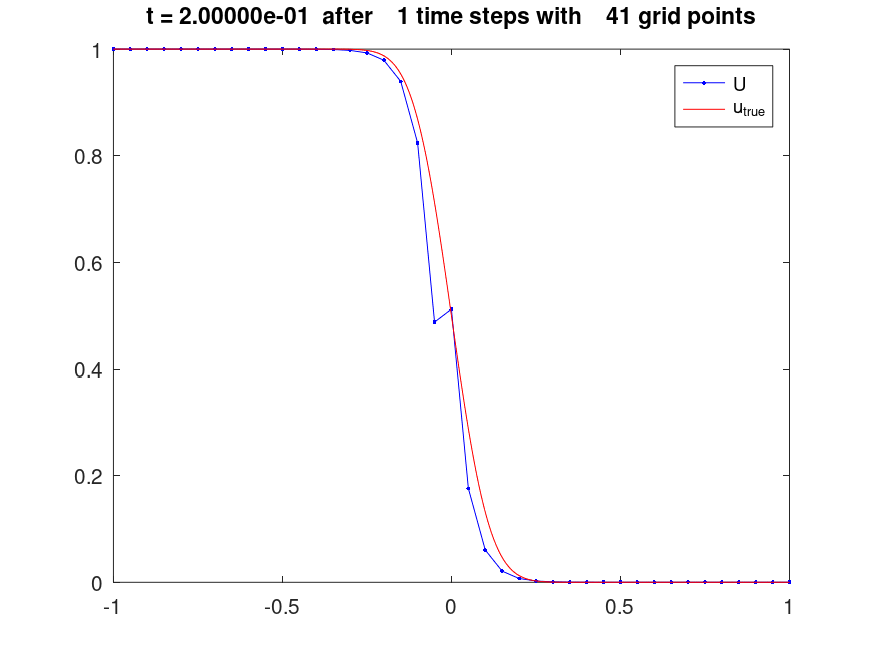
\includegraphics[width=\textwidth]{problem_3ai_heatCN_t-1.png}
                      \caption{$t = 0.2$}
                  \end{subfigure}
                  \hfill
                  \begin{subfigure}[b]{0.4\textwidth}
                      \centering
                      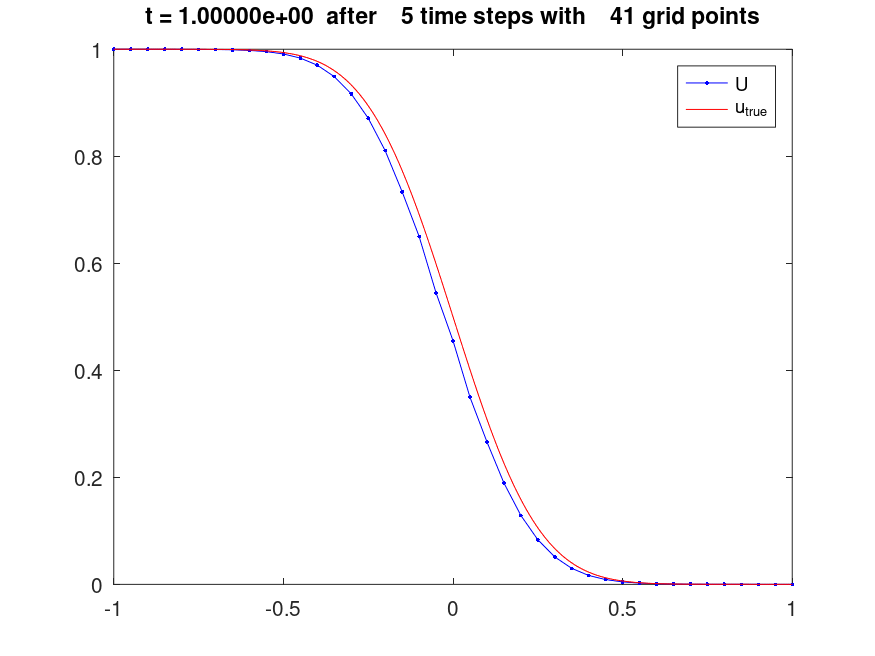
\includegraphics[width=\textwidth]{problem_3ai_heatCN_t-5.png}
                      \caption{$t = 1$}
                  \end{subfigure}
                  \caption[]{CN solution with $\alpha=4$}
              \end{figure*}
              \pagebreak
        \item We start to see somewhat reasonable results when $\alpha < 3$; we observe much better results when $m$ is
              even since odd $m$ forces the approximation to match the point of discontinuity and in turn causes the
              approximation function to skew toward the true solution function value - zero - at $x = 0$.
              \ \\
              
              \begin{figure*}[h]
                  \centering
                  \begin{subfigure}[b]{0.4\textwidth}
                      \centering
                      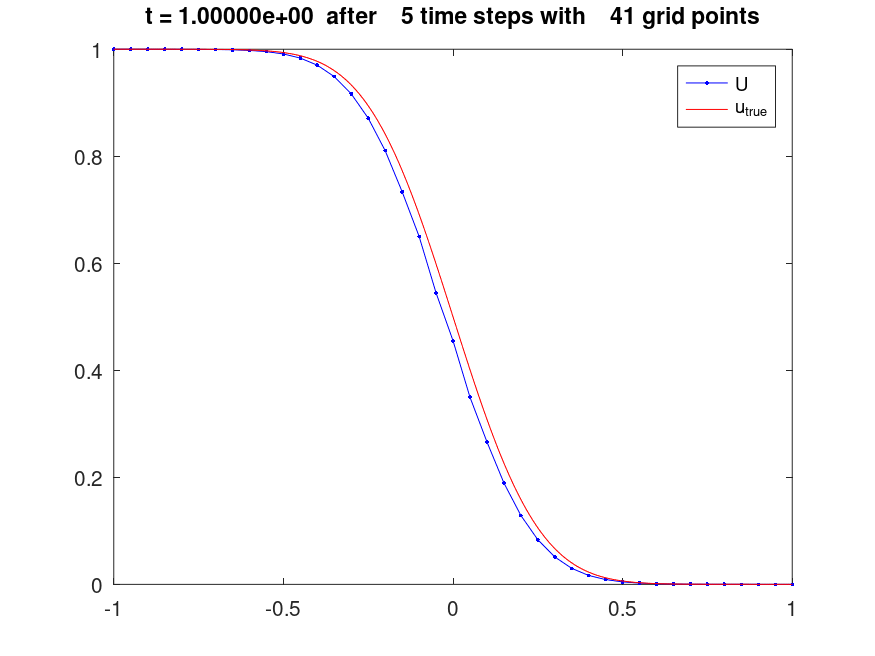
\includegraphics[width=\textwidth]{problem_3aii_m-39_heatCN_t-5.png}
                      \caption{$t = 1$, $m = 39$}
                  \end{subfigure}
                  \hfill
                  \begin{subfigure}[b]{0.4\textwidth}
                      \centering
                      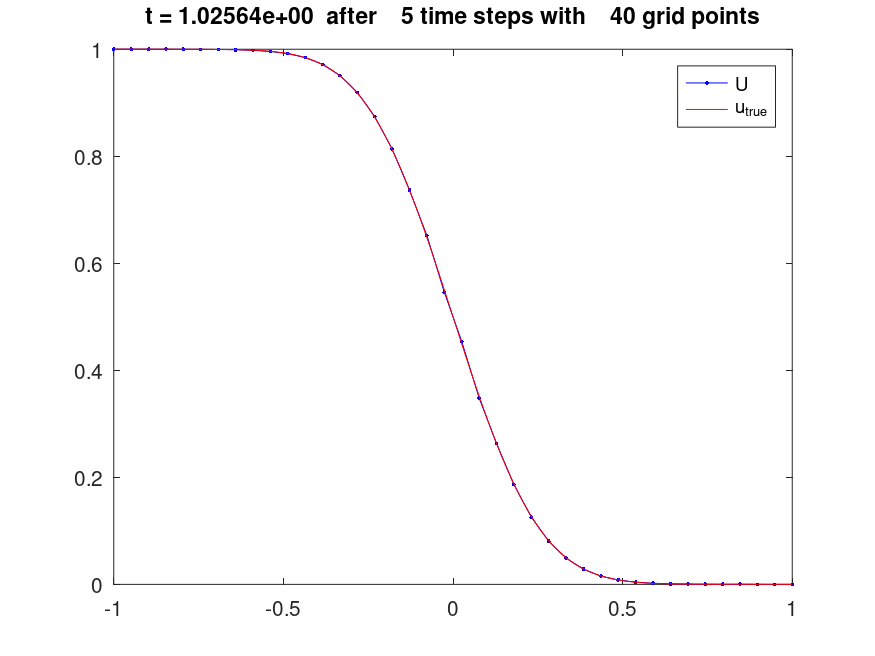
\includegraphics[width=\textwidth]{problem_3aii_m-38_heatCN_t-5.png}
                      \caption{$t = 1$, $m = 38$}
                  \end{subfigure}
                  \caption[]{Comparison between even and odd stencil points}
              \end{figure*}
              
              To determine observed order of accuracy, we let $k = h$ (i.e., $\alpha = 1$) and solve with 
              $m = 18, 38, 48, 78, 98$; the output of \texttt{problem\_3aii.m} given below:

              \begin{figure}[h]
                  \centering
                  \begin{verbatim}
                         h            k          error
                    1.0526e-01   1.0526e-01   9.1383e-03
                    5.1282e-02   5.1282e-02   2.0370e-03
                    4.0816e-02   4.0816e-02   1.2907e-03
                    2.5316e-02   2.5316e-02   5.0210e-04
                    2.0202e-02   2.0202e-02   3.2569e-04
                  
                 Least squares fit gives E(h) = 0.84268 * h^2.01983
                  \end{verbatim}
                  \caption{Output of \texttt{problem\_3aii.m}}
              \end{figure}
              
              The least squares fit from above corresponds to $h$ versus error, and because \linebreak
              $\Delta t = k = h = \Delta x$, we observe that our order of accuracy is 
              $\mathcal{O}\left(h^2 + k^2\right)$.
    \end{enumerate}
    \ \\
\end{solution}